\documentclass[9pt]{beamer}
\usetheme[progressstyle=movCircCnt]{PBEsimple}

\usepackage[T1]{fontenc}
\usepackage[utf8]{inputenc}
\usepackage[portuguese]{babel}
\usepackage{animate}
\usepackage{multicol}
\usepackage{amsfonts}
\usepackage{multirow}
\usepackage{array,booktabs}
\newcommand{\PR}[1]{\ensuremath{\left[#1\right]}}
\newcommand{\PC}[1]{\ensuremath{\left(#1\right)}}
\newcommand{\chav}[1]{\ensuremath{\left\{#1\right\}}}

\title[Bioestatística]{\bf Bioestatística\\
\vspace{.3\baselineskip}}
\subtitle[]{\bf}

\date{ 23 de Março de 2017}
\author[Isolde Previdelli]{
  Isolde Previdelli\\
  \href{itsprevidelli@uem.br}{{\tt itsprevidelli@uem.br \\
isoldeprevidelli@gmail.com \\ \vspace{8mm} \tt \textbf{\LARGE{AULA 5 -
    Medidas de Associação}}}}
}
\institute[PBE/UEM]{}

% % % % % % % % % % % % % % % % % % % % % % % % % % % % % % % % % %

\begin{document}
% Página Título
{\pbebg
\begin{frame}[plain,noframenumbering]
  \titlepage
\end{frame}}

%%%%%%%%%%%%%%
\begin{frame}{Sumário}{}
\tableofcontents
\end{frame}
%%%%%%%%%%%%%%

\section{Etapas na análise de dados}
%\subsection{Etapas na análise de dados}

\begin{frame}{Etapas na análise de dados}{}

\begin{itemize}

\item Coleta de dados
\item Redação dos dados
\item Análise descritiva - univariada
\item Análise comparativa - bivariada
  \begin{itemize}
    \item Medidas de associação
    \item Testes estatísticos
  \end{itemize}
\item Análise multivariada
\item Discussão
\item Conclusão
\end{itemize}

\end{frame}


%\subsection{Análise Bivariada}
\begin{frame}{Etapas na análise de dados}{}


\begin{itemize}
\item Variável resposta
\item Variável independente
\end{itemize}
\indent

Exemplo: Em uma pesquisa o interesse é avaliar se a hipertensão está
relacionada com as variáveis idade e sexo, bem como se estas variáveis
se interagem.

\begin{enumerate}
  \item Variável resposta:
  \item Variáveis Independentes:
\end{enumerate}

lembrando: Trataremos somente o caso em que a variável resposta e as
variáveis independentes são dicotômicas.

\end{frame}



\section{Tabela de contingência 2x2}
\begin{frame}{Tabela de contingência 2x2}{}

%\begin{table}[]
%\caption{Disposição de tabela 2x2 entre doença e exposição}
%\label{my-label}
%\begin{tabular}{llll}
%\multicolumn{1}{c}{}       & \multicolumn{1}{c}{$D_+$} & $D_-$                  & Total \\ \cline{2-3}
%\multicolumn{1}{l|}{$E_+$} & \multicolumn{1}{l|}{a}    & \multicolumn{1}{l|}{b} & a+b   \\ \cline{2-3}
%\multicolumn{1}{l|}{$E_-$} & \multicolumn{1}{l|}{c}    & \multicolumn{1}{l|}{d} & c+d   \\ \cline{2-3}
%Total                      & a+c                       & b+d                    & N
%\end{tabular}
%\end{table}

\begin{figure}[!htb]
    \centering
    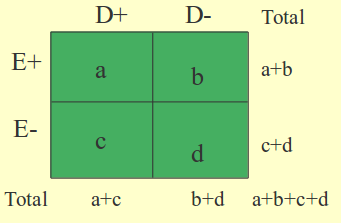
\includegraphics[scale=0.65]{tab.png}
\end{figure}


\end{frame}


\section{Risco Relativo}
\begin{frame}{Risco Relativo}{}

\begin{itemize}
  \item Uma das medidas de associação mais utilizadas em estudos
    clínicos e epidemiológicos é o risco relativo (RR), ou razão de
    riscos. Ele representa uma razão entre estimativas de risco entre os
    indivíduos expostos e não-expostos.
 \item Na prática, utiliza-se a medida de incidência como uma estimativa
   de risco.

\end{itemize}

Olhando para a tabela abaixo, qual seria o risco nos expostos?
E entre os não expostos?\\
$$ Risco_{E_+} = \frac{a}{a+b} $$

$$Risco_{E_-} = \frac{c}{c+d} $$


\begin{figure}[!htb]
    \centering
    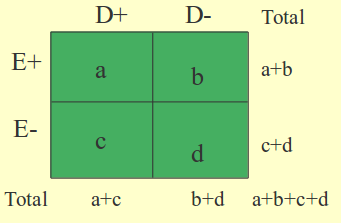
\includegraphics[scale=0.3]{tab.png}
\end{figure}



\end{frame}


%\subsection{Diagrama de caixas - Boxplot}
\begin{frame}{Risco relativo}{}

Portanto,o cálculo do RR, geralmente aplicado em estudo coorte, em uma
tabela 2X2 é dada por:

$$ RR = \frac{Risco_{E_+}}{Risco_{E_-}}$$

\textbf{Interpretação:}\\
Se o risco de uma doença é:

\begin{itemize}
  \item Igual no grupo exposto e não-exposto - $RR=1$
  \item Maior no grupo exposto - $RR > 1$ (fator de risco)
  \item Menor no grupo exposto - $RR < 1$ (fator de proteção)
\end{itemize}


\end{frame}


\subsection{Medidas de risco absoluto e relativo}
\begin{frame}{Medidas de risco absoluto e relativo}{}

\textbf{Dependem do tipo de estudo:}\\

\begin{itemize}
\item Estudo coorte, ensaios controlados e aleatorizados:
  \begin{itemize}
    \item Medidas relativas e absolutas de risco.
  \end{itemize}
  \item Estudos de caso-controle:
  \begin{itemize}
    \item Razão de chances.
  \end{itemize}
\end{itemize}
\end{frame}


\begin{frame}{Medidas de risco absoluto e relativo}{}


\begin{figure}[!htb]
    \centering
    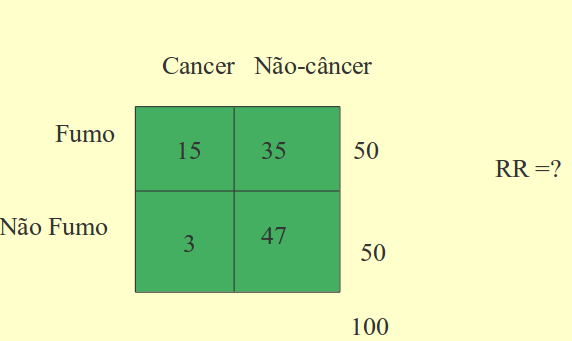
\includegraphics[scale=0.5]{tab2.png}
\end{figure}



\end{frame}


\begin{frame}{Exercício}{}

\begin{block}{blue}{}

Uma pesquisa com $531$ pessoas sobre incidência de ferimentos faciais em
acidentes com motocicleta, com e sem uso de capacetes, revelou os
seguintes dados:\\
\indent

Em $113$ pacientes com capacete apenas $30$ apresentaram ferimentos da
face e, no outro grupo, $182$. No presente estudo, qual o risco relativo
do paciente sem capacete apresentar lesão facial?
\end{block}



\end{frame}






\section{Odds ratio - Razão de chances}
\begin{frame}{Odds ratio - Razão de chances}{}

\begin{itemize}
  \item Nos estudos caso-controle não é possível estimar diretamente o
    risco, pois não "fixamos" o número de pessoas expostas
  \item Assim utiliza-se uma outra abordagem, que é o cálculo das
    chances(\textit{odds}) de exposição entre os casos em comparação com
    as chances de exposição entre os controles.
  \item Em uma tabela $2x2$, o cálculo da \textit{odds-ratio} é dada por:

\end{itemize}
\begin{figure}[!htb]
    \centering
    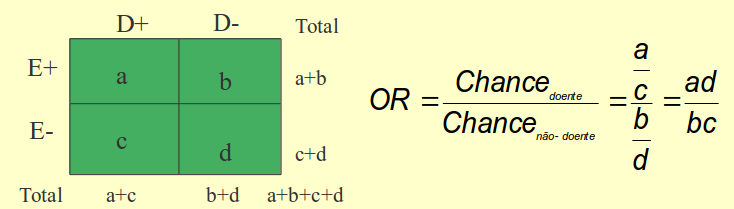
\includegraphics[scale=0.4]{tab3.png}
  \end{figure}
\end{frame}



\begin{frame}{Interpretação da razão de chance}{}

\textbf{Se a razão de chance de uma doença é:}


\begin{itemize}
\item Igual no grupo exposto e não- exposto - $OR = 1$
\item maior no grupo exposto e não- exposto - $OR > 1$ (fator de risco)
\item Menor no grupo exposto e não- exposto - $OR < 1$ (fator de proteção)
\end{itemize}



\end{frame}


%\subsection{Diagrama de dispersão}
\begin{frame}{Odds ratio - razão de chance}{}

\begin{figure}[!htb]
    \centering
    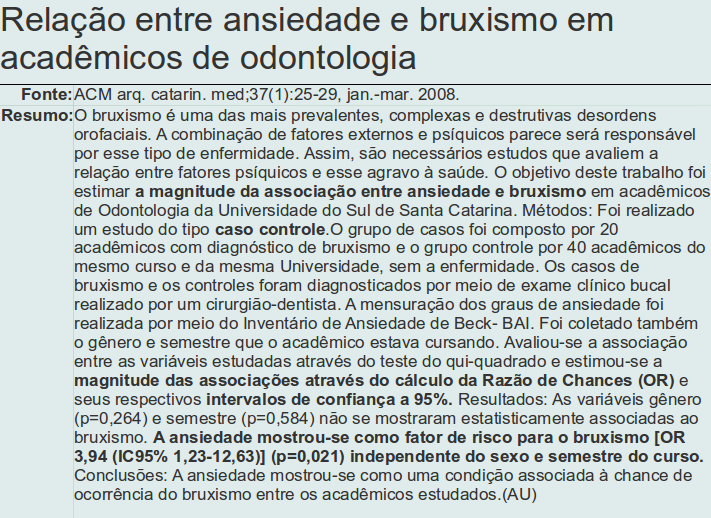
\includegraphics[scale=0.385]{fig_odss.png}
  \end{figure}
\end{frame}


\begin{frame}{Odds ratio - razão de chance}{}

\begin{figure}[!htb]
    \centering
    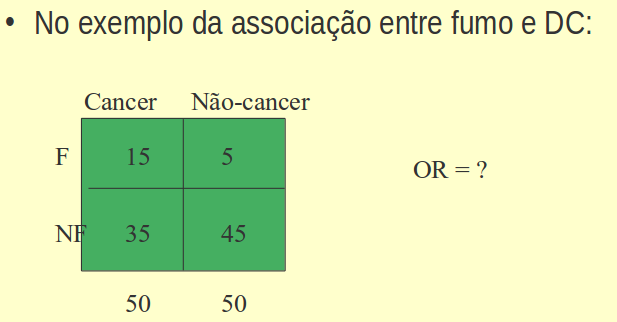
\includegraphics[scale=0.45]{odds.png}
  \end{figure}
\end{frame}



\begin{frame}{Odds ratio - razão de chance}{Exercício}


Um estudo de acidentes de automóvel, entre 736 motoristas com e sem uso
de telefone celular, acusou os seguintes dados: entre os 310 motoristas
usavam telefone ocorreram 28 acidentes e, entre os 426 que não usavam
telefone, ocorreram 19. Qual a razão de chance de ocorrer acidente com
uso do aparelho?\\
\indent

Num estudo com 600 motoristas acidentados, testou-se a eficiência do
uso do cinto de segurança na prevenção de lesões da coluna vertebral
cervical, em colisões frontais, em alta velocidade.
Entre os 546 motoristas que usavam cinto apenas 13 apresentaram lesão e,
entre os demais, ocorreram 8 lesões. Qual a razão de chance de ocorrer
lesão sem o uso do cinto de segurança?\\
\indent


\textbf{Ler Risco Relativo e Razão de chances no Soares – 7.4.2 e 7.4.2
– p. 246}

\end{frame}


\begin{frame}{Entendendo a diferença entre Risco e Chance}{}

\begin{itemize}
\item Risco de doença no grupo exposto:
  \begin{itemize}
    \item Probabilidade da doença entre os expostos, $Risco_{exposto} =
 \frac{a}{a+b}$
  \end{itemize}

    \item Chance do exposto:
  \begin{itemize}
    \item Razão entre os expostos com a doença e os expostos sem a
      doença, $Chance_{exposto} = \frac{a}{b}$
  \end{itemize}

\end{itemize}

\end{frame}


%\section{Medidas de associação}
\begin{frame}{Medidas de associação}{}

\begin{block}{red}{}

%\begin{table}[!htb]
%\begin{tabular}{ll}
%\hline
%Tipo de estudo & Medidas de associação \\
%\hline
%Coorte         & Risco Relativo \\
%Caso-controle  & Odds ratio \\
%Ensaio clínico & Risco Relativo
%\hline
%\end{tabular}
%\end{table}


\begin{table}[!htb]
\centering
%\caption{My caption}
%\label{my-label}
\begin{tabular}{ll}
\hline
\multicolumn{1}{c}{Tipo de estudo} & \multicolumn{1}{c}{Medidas de associação} \\ \hline
Coorte                               & Risco relativo                             \\
Caso-controle                        & Odss ratio                                 \\
Ensaio clínico                       & Risco relativo                             \\ \hline
\end{tabular}
\end{table}



\end{block}
\end{frame}





%%%%%%%%%%%%%%%

{\pbebg
\begin{frame}[plain,noframenumbering]

\finalpage{\begin{figure}[!htb]
    \centering
   
\includegraphics[scale=0.21]{word.jpg}
  \end{figure}
Obrigada!}

\end{frame}}
%%%%%%%%%%%%%%%%
\end{document}